\begin{figure}[!t]
  \centering
  \begin{minipage}{0.88\linewidth}
    \captionsetup[subfigure]{font=small,skip=4pt,justification=centering}
    \begin{subfigure}{\linewidth}
      \centering
      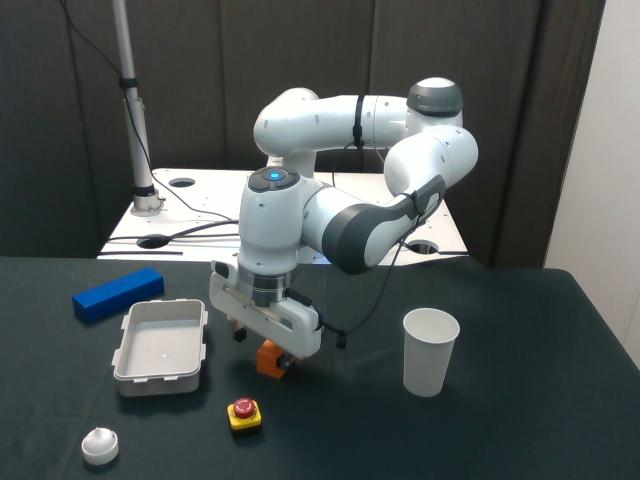
\includegraphics[width=0.326\linewidth]{assets/real_robot/panda_pick/front_059.jpg}\hfill
      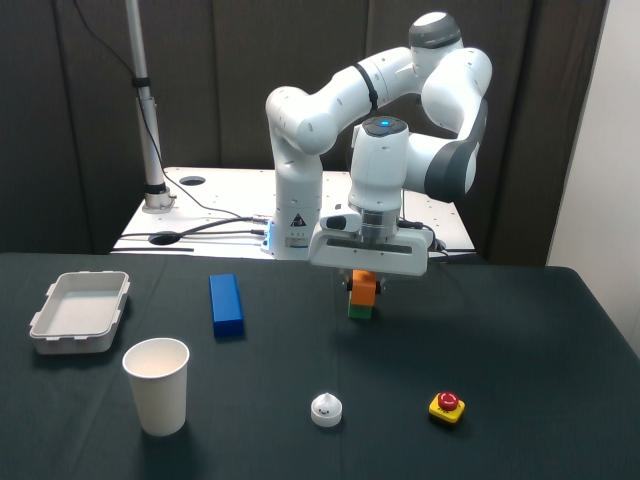
\includegraphics[width=0.326\linewidth]{assets/real_robot/cube_stack/front_011.jpg}\hfill
      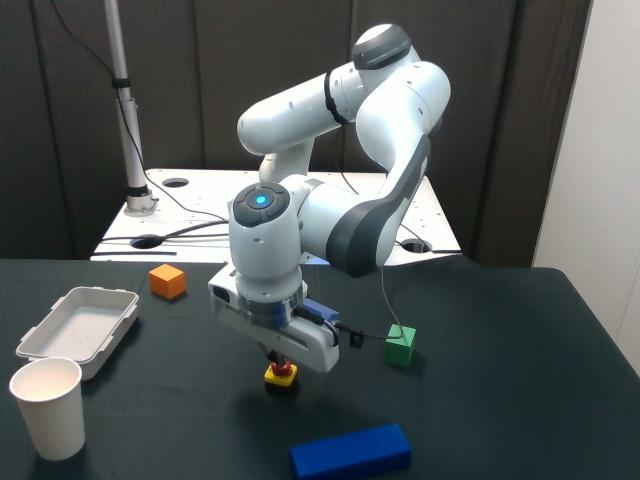
\includegraphics[width=0.326\linewidth]{assets/real_robot/press_button/front_010.jpg}
      \caption{Real Robot}
      \label{fig:environments-real}
    \end{subfigure}

    \medskip
    \begin{subfigure}[t]{0.482\linewidth}
      \centering

      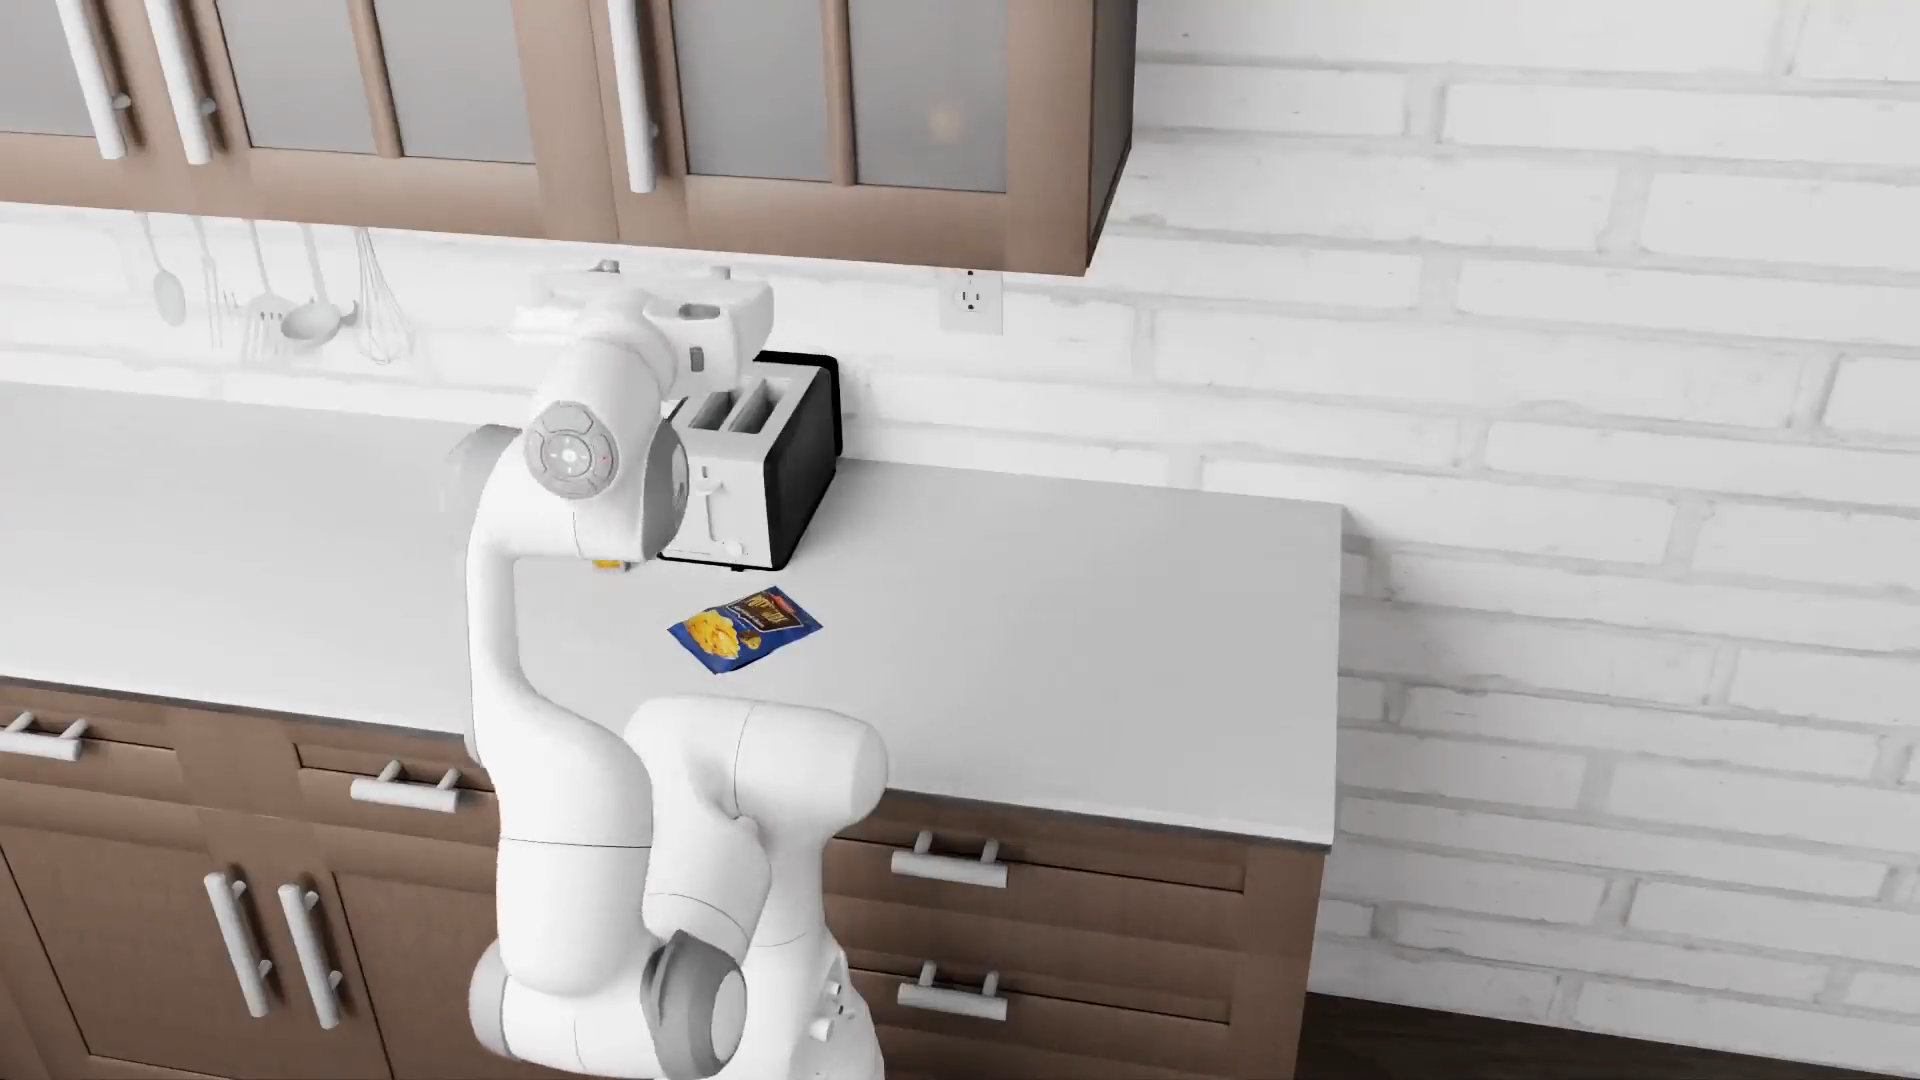
\includegraphics[width=0.489\linewidth,trim={240 0 240 0},clip]{assets/environments/robocasa.png}\hfill
      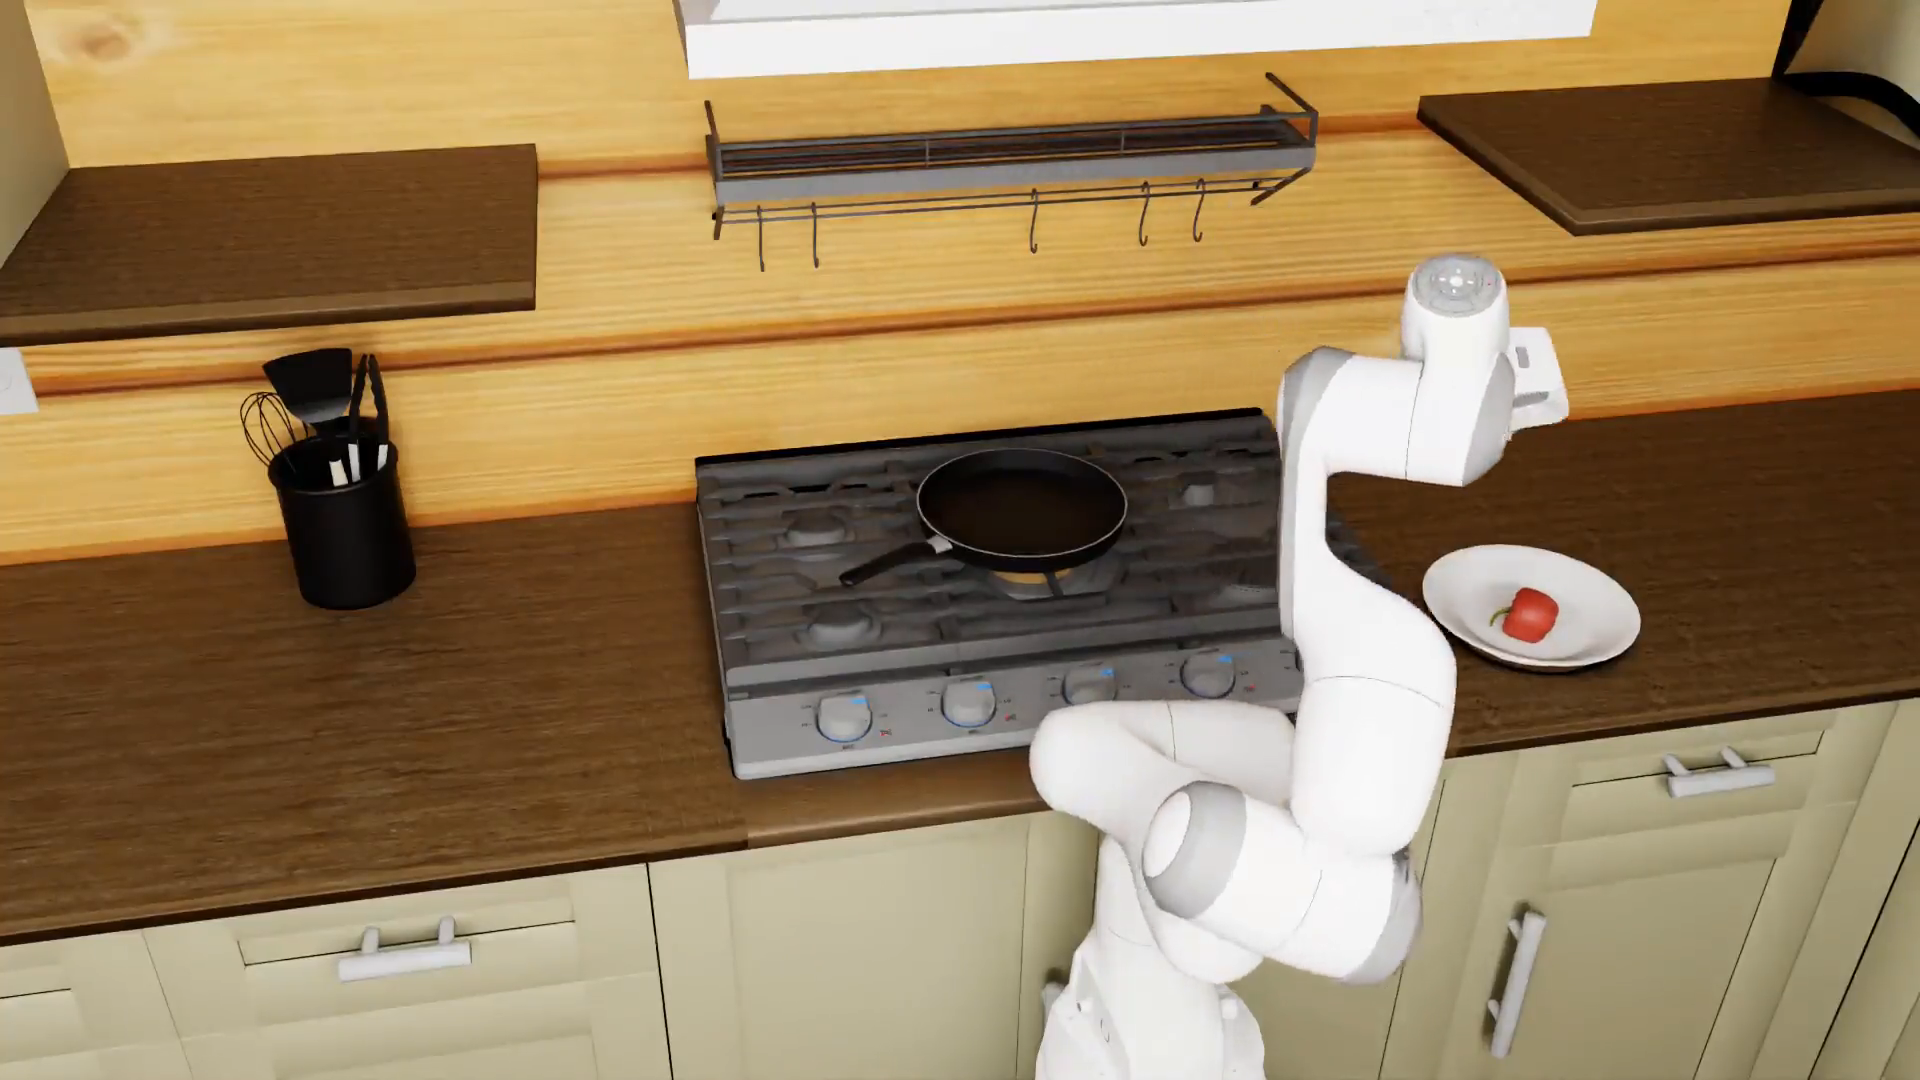
\includegraphics[width=0.489\linewidth,trim={350 0 130 0},clip]{assets/environments/robocasa-pnp.png}
      \caption{RoboCasa}
      \label{fig:environments-robocasa}
    \end{subfigure}\hfill
    \begin{subfigure}[t]{0.482\linewidth}
      \centering

      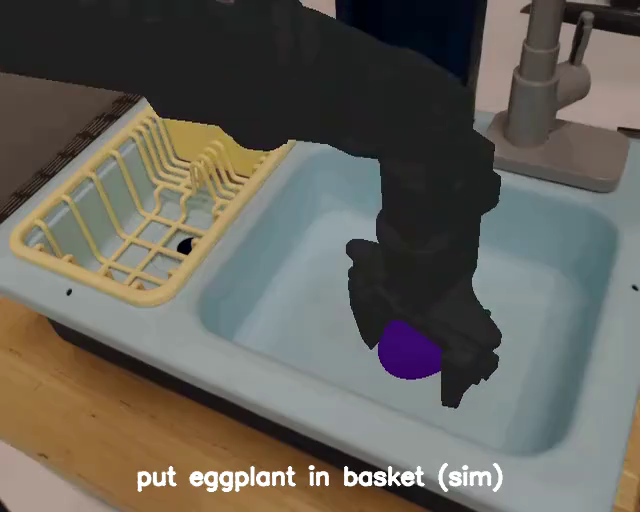
\includegraphics[width=0.489\linewidth,trim={20 62 20 0},clip]{assets/environments/bridge.png}\hfill
      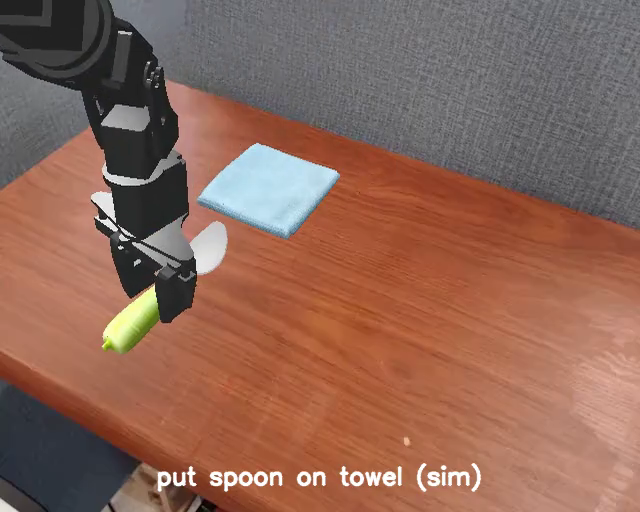
\includegraphics[width=0.489\linewidth,trim={20 62 20 0},clip]{assets/environments/bridge-spoon.png}
      \caption{SimplerEnv Bridge}
      \label{fig:environments-bridge}
    \end{subfigure}
  \end{minipage}
  \caption{Evaluation environments. (a) Real robot: pick and place, cube stacking, and button pressing. (b) RoboCasa~\citep{nasiriany2024robocasa}: cabinet interaction and pick and place. (c) SimplerEnv Bridge~\citep{li2025simpler}: eggplant in basket and spoon on towel. Scenes are ordered left to right within each group; simulation images are from official project demonstrations.}
  \label{fig:environments}
\end{figure}
